\newpage
\section{Pseudoalgoritmos.}
En esta sección vamos a ver algunos pseudoalgoritmos referentes a los algoritmos que hemos implementado. Nos vamos a centrar en aquellos que tienen mayor complejidad e interés, sin entrar en gran detalle. Es importante destacar que estos algoritmos no están establecidos como tales, sino que los hemos implementando intentando reflejar los conceptos matemáticos que hemos ido viendo. \\

En concreto, vamos a ver los pseudoalgoritmos para el algoritmo de Dehornoy (que descomponemos en varios algoritmos auxiliares), el algoritmo que nos permite comprobar si dos trenzas dadas (o sus cierres) son o no equivalentes entre sí y el algoritmo que nos permite comprobar si una trenza dada (o su cierre) es equivalente a la trenza trivial.\\

\begin{center}
	\textbf{Algoritmo Dehornoy para trenzas.}
\end{center} 
Vamos a ir viendo los algoritmos auxiliares y concluiremos con el propio algoritmo de Dehornoy. Recordemos que este algoritmo se explica con detalle en la sección \ref{deh}.\\

Creamos el método Simplifica mediante el cuál eliminamos ocurrencias de tipo $\sigma_{i}^{e}\sigma_{i}^{-e}$, siendo $ e \in$ \{-1,1\}, de una palabra que representa a cierta trenza. 

\begin{alg}
	\textbf{Algoritmo Simplifica}(índices\_braid)\\
	ENTRADA: índices\_braid (cadena de enteros que representa los cruces de una trenza)\\
	SALIDA: \hspace{0.4cm} braid\_aux (cadena auxiliar para mejor representacion visual) \\
    \hspace*{2.2cm} nueva\_braid (cadena de enteros que representa los cruces de la trenza tras eliminar dos cruces consecutivos opuestos)\\
    \hspace*{2.2cm} encontrado (bool para indicar si se produce simplificación)
	
	\lstset{language=Matlab, breaklines=true, basicstyle=\ttfamily\small ,numbers=left, stepnumber=1, numberstyle=\color{blue}, literate={á}{{\'a}}1
		{í}{{\'i}}1
		{é}{{\'e}}1
		{ú}{{\'u}}1
		{ó}{{\'o}}1
		{ñ}{{\~n}}1}
\begin{lstlisting}
   Recorro los cruces de índices_braid
   Si hay dos cruces seguidos con signos opuestos, creo una copia de índices_braid y elimino dichos cruces. 
\end{lstlisting}
\end{alg}

Haciendo uso del siguiente algoritmo podremos encontrar las posiciones que delimitan un $\sigma_{minimo}$-handle.
\begin{alg}
	\textbf{Algoritmo encuentra\_handle}(índices\_braid, mínimo)\\
	ENTRADA: índices\_braid (cadena de enteros que representa los cruces de una trenza)\\
	\hspace*{2.2cm} mínimo (generador de handle a encontrar) \\
	SALIDA: \hspace{0.4cm} pos1 (posición inicial del handle encontrado) \\
	\hspace*{2.2cm} pos2 (posición final del handle encontrado)
	
	\lstset{language=Matlab, breaklines=true, basicstyle=\ttfamily\small ,numbers=left, stepnumber=1, numberstyle=\color{blue}, literate={á}{{\'a}}1
		{í}{{\'i}}1
		{é}{{\'e}}1
		{ý}{{\'y}}1
		{ú}{{\'u}}1
		{ó}{{\'o}}1
		{ñ}{{\~n}}1}
\begin{lstlisting}
   Recorro los cruces de índices_braid
   Si hay un cruce generado por el elemento mínimo, me quedo con esa posición como pos1 y su signo. Si no finalizo.
   Si encuentro un cruce generado por el elemento mínimo con signo opuesto, me quedo con esa posición como pos2.
\end{lstlisting}
\end{alg}

\bigskip
Haciendo uso del algoritmo reduccion\_base aplicamos una reducción local a la trenza representada por indices\_braid sobre el $\sigma_{minimo}$-handle que está situado entre las posiciones pos1 y pos2. Es importante destacar el hecho de que este $\sigma_{minimo}$-handle  no contiene $\sigma_{minimo+1}$-handle. Este detalle lo controlamos en el algoritmo Dehornoy que veremos posteriormente. \\

\begin{alg}
	\textbf{Algoritmo reduccion\_base}(índices\_braid, mínimo, pos1, pos2 )\\
	ENTRADA: índices\_braid (cadena de enteros que representa los cruces de una trenza)\\
	\hspace*{2.2cm} mínimo (generador de handle) \\
	\hspace*{2.2cm} pos1 (posición inicial del handle) \\
	\hspace*{2.2cm} pos2 (posición final del handle)\\
	SALIDA: \hspace{0.4cm} braid\_aux2 (cadena auxiliar para mejor representación visual) \\
	\hspace*{2.2cm} nuevo (cadena de enteros que representa los cruces de la trenza tras aplicar la reducción local al $\sigma_{minimo}$-handle entre pos1 y pos2)\\
	\hspace*{2.2cm} simplificado2 (bool auxiliar para mejor representación visual)
	
	\lstset{language=Matlab, breaklines=true, basicstyle=\ttfamily\small ,numbers=left, stepnumber=1, numberstyle=\color{blue}, literate={á}{{\'a}}1
		{í}{{\'i}}1
		{é}{{\'e}}1
		{ú}{{\'u}}1
		{ó}{{\'o}}1
		{ñ}{{\~n}}1}
\begin{lstlisting}
   Creo vector_auxiliar
   Recorro los cruces de índices_braid desde pos1 hasta pos2
   Si hay un cruce generado por el elemento (mínimo+1) añado a vector_auxiliar los 3 cruces correspondientes del algoritmo. Si no, añado el mismo cruce. 
   Creo vector_nuevo con los elementos desde inicio de índices_braid hasta pos1, vector_auxiliar, y los elementos desde pos2 hasta final de indices_braid.
   Si índices_braid y vector_auxiliar tienen distinto tamaño, asigno a braid_aux2 una cadena con ciertos ceros para mejor visualización.
\end{lstlisting}
\end{alg}


Estos algoritmos auxiliares no se proporcionan para uso directo al usuario ya que el realmente interesante es el algoritmo de Dehornoy, pero sí podrían ser usados. Veamos entonces el algoritmo de Dehornoy.\\

\begin{alg}
	\textbf{Algoritmo dehornoy}(br, N\_cortes, Radio, representar)\\
	ENTRADA: br (trenza)\\
	\hspace*{2.2cm} N\_cortes (número de cortes de las cadenas de la trenza)\\
	\hspace*{2.2cm} Radio (radio de las cadenas de la trenza)\\
	\hspace*{2.2cm} representar (bool para representar las equivalencias de la trenza)\\
	SALIDA: \hspace{0.4cm} es\_trivial (bool que nos indica si la trenza dada es o no trivial) \\
	\hspace*{2.2cm} trenza\_final (cadena de enteros que representa a la trenza reducida equivalente a br)
	
	\lstset{language=Matlab, breaklines=true, basicstyle=\ttfamily\small ,numbers=left, numbersep=-2pt, numberstyle=\color{blue}, literate={á}{{\'a}}1
		{í}{{\'i}}1
		{é}{{\'e}}1
		{ú}{{\'u}}1
		{ó}{{\'o}}1
		{ñ}{{\~n}}1}
\begin{lstlisting}
   Si número_argumentos=1 -> N_cortes=20, Radio=0.5, representar=1.
   índices_braid = cadena de enteros que representa a la trenza
   Si br tiene cadenas a la derecha triviales, las eliminamos visualmente.
   Mientras queden handles en la trenza dada...
	 Obtenemos la palabra libremente reducida de indices_braid.
	 Si no se produce reduccion...
	   mínimo = generador principal de índices_braid.
	   [pos1,pos2]=encuentra_handle(índices_braid,mínimo)
	   Si pos1 y pos2 son posiciones válidas....
		   Busco primer subhandle a realizar en el handle.
		   Actualizo pos1 y pos2
		   Aplico reduccion_base a dicho subhandle.
	 Creo matriz con secuencia de palabras generadas en el proceso
   Si representar, muestro las trenzas usando dicha matriz.			   
\end{lstlisting}
\end{alg}

Finalmente cabe comentar que el algoritmo de Dehornoy se podrá aplicar sobre trenzas cerradas. El proceso que se realizará internamente será exactamente el mismo que para trenzas, ya que el cerrar la trenza no aporta información nueva para el algoritmo de Dehornoy. Por este mismo motivo, a la hora de realizar la visualización del algoritmo de Dehornoy sobre una trenza cerrada, veremos las transformaciones sobre la trenza y no sobre la trenza cerrada. \\

\bigskip
\begin{center}
	\textbf{Algoritmo de equivalencia para trenzas.}
\end{center} 
Para ver si dos trenzas dadas son equivalentes o no entre sí, vamos a implementar algunos de los invariantes que vimos para trenzas. En concreto, vamos a estudiar los invariantes exponente y permutación. Si con estos invariantes no conseguimos analizar la equivalencia de las trenzas, vamos a aplicar el algoritmo de Dehornoy que hemos visto anteriormente. \\

\begin{alg}
	\textbf{Algoritmo equivalentes}(br1,br2,explicación)\\
	ENTRADA: br1 (trenza1)\\
	\hspace*{2.2cm} br2 (trenza2)\\
	\hspace*{2.2cm} explicación (bool para mostrar mensajes explicativos)\\
	SALIDA: \hspace{0.4cm} equi (bool para indicar si br1 y br2 son o no equivalentes)
	
	\lstset{language=Matlab, breaklines=true, basicstyle=\ttfamily\small ,numbers=left, stepnumber=1, numberstyle=\color{blue}, literate={á}{{\'a}}1
		{í}{{\'i}}1
		{é}{{\'e}}1
		{ú}{{\'u}}1
		{ó}{{\'o}}1
		{ñ}{{\~n}}1}
\begin{lstlisting}
   Si número_argumentos=2 -> explicación=0.
   Obtengo exponente de ambas trenzas.
   Si son distintos -> No son equivalentes. Finalizo
   Obtengo permutación de ambas trenzas.
   Si son distintas -> No son equivalentes. Finalizo
   Genero trenza_auxiliar = br1inver(br2).
   Aplico Dehornoy a trenza_auxiliar y obtengo final_braid.
   Si final_braid no es vacia -> No son equivalentes. 
   Si no -> Si explicacion=1 -> represento secuencia de trenzas de dehornoy.
    
\end{lstlisting}
\end{alg}

\bigskip
\begin{center}
	\textbf{Algoritmo de equivalencia para trenzas cerradas.}
\end{center} 
Para analizar la equivalencia de dos trenzas cerradas, vamos a apoyarnos en el algoritmo de equivalencia de las trenzas sin cerrar que hemos visto anteriormente. Además haremos uso de varios algoritmos auxiliares. En concreto, hemos implementado los movimientos de Markov que vimos en la sección \ref{Markov}.\\

Sabemos que el movimiento 1 de Markov puede eliminar o añadir cruces. Siempre intentaremos eliminar cruces, mientras que para añadir cruces se tiene que solicitar explícitamente. Lo hacemos así para que las trenzas no aumenten en número de cruces salvo que no quede más opción. \\ 

\begin{alg}
	\textbf{Algoritmo MV1}(br\_c, completo)\\
	ENTRADA: br\_c (trenza cerrada)\\
	\hspace*{2.2cm} completo (bool para indicar si se desean añadir cruces)\\
	SALIDA: \hspace{0.4cm} a2 (trenza cerrada tras aplicar Movimiento1 eliminando de Markov.) 
	
	\lstset{language=Matlab, breaklines=true, basicstyle=\ttfamily\small ,numbers=left, stepnumber=1, numberstyle=\color{blue}, literate={á}{{\'a}}1
		{í}{{\'i}}1
		{é}{{\'e}}1
		{ú}{{\'u}}1
		{ó}{{\'o}}1
		{ñ}{{\~n}}1}
\begin{lstlisting}
   Si número_argumentos=1 -> completo=0.
   Si el primer cruce de br_c es opuesto al último cruce de br_c -> a2 = br_c sin dichos cruces.
   Si no -> Si completo... 
     Obtengo cruce de mayor índice (índice m).
     Añado cruces opuestos de índice m a principio y final de br_c.
      
\end{lstlisting}
\end{alg}

\begin{alg}
	\textbf{Algoritmo MV2}(br\_c)\\
	ENTRADA: br\_c (trenza cerrada)\\
	SALIDA: \hspace{0.4cm} a3 (trenza cerrada tras aplicar Movimiento2 de Markov.) 
	
	\lstset{language=Matlab, breaklines=true, basicstyle=\ttfamily\small ,numbers=left, stepnumber=1, numberstyle=\color{blue}, literate={á}{{\'a}}1
		{í}{{\'i}}1
		{é}{{\'e}}1
		{ú}{{\'u}}1
		{ó}{{\'o}}1
		{ñ}{{\~n}}1}
\begin{lstlisting}
   Mientras br_c cambie de cruces...
      Si br_c tiene un solo cruce -> a3=trenza cerrada trivial. Finalizo.
      Obtengo cruce de mayor indice (indice m). 
      Si se encuentra solo una vez en br_c
         Si a izquerda o derecha del cruce no tenemos cruces con índice m-1 -> a3=br_c sin dicho cruce.
         
\end{lstlisting}
\end{alg}

Para implementar este algoritmo de equivalencia entre trenzas cerradas hemos analizado en primer lugar los invariantes básicos de ambas trenzas. Si no obtenemos una respuesta de equivalencia  o no equivalencia, pasamos a ver el polinomio de Alexander de ambas trenzas cerradas. Una vez analizados los invariantes que hemos estudiado, vamos a ir realizando transformaciones de equivalencia sobre la trenza cerrada generada por el producto de la trenza inicial y la inversa de la segunda trenza. \\

Ya sabemos que ir haciendo transformaciones de equivalencia sobre una trenza cerrada para ver si es o no equivalente a la trenza cerrada trivial puede conllevar a una serie indefinida de movimientos. \\

La idea que hemos llevado a cabo consiste en aplicar el Movimiento 1 de Markov, el algoritmo de Dehornoy a la trenza cerrada que obtenemos, el Movimiento 2 de Markov y de nuevo el algoritmo de Dehornoy. Si en alguna de estas transformaciones conseguimos saber si la trenza cerrada es o no equivalente a la trivial, finalizamos el proceso. En caso contrario, realizaremos el mismo proceso un número delimitado de veces. \\

\newpage
\begin{alg}
	\textbf{Algoritmo equivalentes}(br1,br2,explicación)\\
	ENTRADA: br1 (trenza cerrada 1)\\
	\hspace*{2.2cm} br2 (trenza cerrada 2)\\
	\hspace*{2.2cm} explicacioó (bool para mostrar mensajes explicativos)\\
	SALIDA: \hspace{0.4cm} equi (bool para indicar si br1 y br2 son o no equivalentes)
	
	\lstset{language=Matlab, breaklines=true, basicstyle=\ttfamily\small ,numbers=left, stepnumber=1, numberstyle=\color{blue}, literate={á}{{\'a}}1
		{í}{{\'i}}1
		{é}{{\'e}}1
		{ú}{{\'u}}1
		{ó}{{\'o}}1
		{ñ}{{\~n}}1}
\begin{lstlisting}
   Si número_argumentos=2 -> explicación=0.
   Si el número de enlaces de br1 y de br2 son distintos -> No son equivalentes. Finalizo
   Si equivalentes@trenza(br1,br2) son equivalentes -> sus cierres son equivalentes.
   Si no ->   
   	Obengo polinomio de Alexander de ambas trenzas.
	Si son iguales salvo signo -> No sabemos si son o no equivalentes. equi <- 2.
	Sino -> No son equivalentes.
   Si equi=2
    Creo trenza cerrada br = br1inver(br2)
    Mientras número_iteraciones < limite(establecido a 3)
	    a1 = Aplico MV1 a br.
	    [es_trivial2,a2] = Aplico dehornoy a trenza cerrada a1. 
	    Si es_trivial2 -> Finalizo.
	    a3 = Aplico MV2 a trenza cerrada a2.
	    [es_trivial4,a4] = Aplico dehornoy a trenza cerrada a3. 
	    Si es_trivial4 -> Finalizo.
	    Si no ha cambiado br, a4 = Aplico MV1 completo a br. 
	   
\end{lstlisting}
\end{alg}

\begin{center}
	\textbf{Algoritmo para ver trivialidad de trenza.}
\end{center} 
Tanto para ver la trivialidad de una trenza como la trivialidad de una trenza cerrada vamos a usar la misma idea que será hacer uso de los algoritmos de equivalencia entre la trenza dada y la trenza trivial. Veámoslos:

\begin{alg}
	\textbf{Algoritmo es\_trivial}(br,explicación)\\
	ENTRADA: br (trenza)\\
	\hspace*{2.2cm} explicación (bool para mostrar mensajes explicativos)\\
	SALIDA: \hspace{0.4cm} equi (bool para indicar si br es o no equivalente a la trenza trivial)
	
	\lstset{language=Matlab, breaklines=true, basicstyle=\ttfamily\small ,numbers=left, stepnumber=1, numberstyle=\color{blue}, literate={á}{{\'a}}1
		{í}{{\'i}}1
		{é}{{\'e}}1
		{ú}{{\'u}}1
		{ó}{{\'o}}1
		{ñ}{{\~n}}1}
\begin{lstlisting}
   Si número_argumentos=1 -> explicación=0.
   Creo br2 = trenza trivial. 
   Aplico algoritmo equivalentes para br y br2.
\end{lstlisting}
\end{alg}

\begin{center}
	\textbf{Algoritmo para ver trivialidad de trenza cerrada.}
\end{center} 

\begin{alg}
	\textbf{Algoritmo es\_trivial}(br\_c,explicación)\\
	ENTRADA: br\_c (trenza cerrada)\\
	\hspace*{2.2cm} explicación (bool para mostrar mensajes explicativos)\\
	SALIDA: \hspace{0.4cm} equi (bool para indicar si br\_c es o no equivalente a la trenza cerrada trivial)
	
	\lstset{language=Matlab, breaklines=true, basicstyle=\ttfamily\small ,numbers=left, stepnumber=1, numberstyle=\color{blue}, literate={á}{{\'a}}1
	{í}{{\'i}}1
	{é}{{\'e}}1
	{ú}{{\'u}}1
	{ó}{{\'o}}1
	{ñ}{{\~n}}1}
\begin{lstlisting}
   Si número_argumentos=1 -> explicación=0.
   Creo br2_c = trenza cerrada trivial. 
   Aplico algoritmo equivalentes para br_c y br2_c.
\end{lstlisting}
\end{alg}

\newpage

Una vez hemos visto los algoritmos más relevantes enfocados a los aspectos matemáticos que hemos ido desarrollando a lo largo de este proyecto, vamos a centrarnos en el algoritmo de representación de trenzas y trenzas cerradas que hemos creado. Cabe comentar que estos algoritmos han ido pasando por distintas versiones hasta obtener una versión con la que poder representar las transiciones de trenzas para el algoritmo de Dehornoy de la forma más elegante e intuitiva posible. 

 \begin{center}
 	\textbf{Algoritmo para representar una trenza.}
 \end{center} 
 Vamos a ir viendo algunos algoritmos auxiliares que hemos creado y concluiremos con el algoritmo de representación de una trenza. \\
 En primer lugar, creamos un método que nos permita representar un tubo de ciertas dimensiones (radio y número de cortes) con centro una función dada por las coordenadas x, y, z. Estos tubos formarán las cadenas de la trenza, pero ahora mismo sería un tubo sobre una función cualquiera, veámoslo:
 
 \begin{alg}
 	\textbf{Algoritmo tubep}(x,y,z,N,R)\\
 	ENTRADA: x (coordenada x de la función)\\
 	\hspace*{2.2cm} y (coordenada y de la función)\\
 	\hspace*{2.2cm} z (coordenada z de la función)\\
 	\hspace*{2.2cm} N (número de cortes que tendrá el tubo (cadena de la trenza))\\
 	\hspace*{2.2cm} R (Radio del tubo (cadena de la trenza))
 	
 	\lstset{language=Matlab, breaklines=true, basicstyle=\ttfamily\small ,numbers=left, stepnumber=1, numberstyle=\color{blue}, literate={á}{{\'a}}1
 		{í}{{\'i}}1
 		{é}{{\'e}}1
 		{ú}{{\'u}}1
 		{ó}{{\'o}}1
 		{ñ}{{\~n}}1}
\begin{lstlisting}
   Obtenemos matrices con puntos circulares con centro la función de entrada.
   Creamos una superficie a partir de dichas matrices.
   Leemos imagen de textura.
   Aplicamos la imagen a la superficie.
   Establecemos puntos de iluminación.
   
\end{lstlisting}
 \end{alg}
 
 A continuación, vamos a ver el algoritmo que hemos creado para obtener la forma que presenta una sección de una cadena de una trenza al producirse un cruce. Con este algoritmo únicamente obtenemos las coordenadas de la función que tiene dicha forma. Hemos decidido darle esta parametrización a la función para que visualmente quede lo mejor posible. 
 
  \begin{alg}
  	\textbf{Algoritmo giro\_base}()\\
  	SALIDA: \hspace{0.4cm} x (vector de coordenadas x de una función para generar una de las dos partes de un cruce)\\
  	\hspace*{2.2cm} y (vector de coordenadas y de una función para generar una de las dos partes de un cruce)\\
  	\hspace*{2.2cm} z (vector de coordenadas z de una función para generar una de las dos partes de un cruce)
  	
  	\lstset{language=Matlab, breaklines=true, basicstyle=\ttfamily\small ,numbers=left, stepnumber=1, numberstyle=\color{blue}}
\begin{lstlisting}
   x <- vector con valores nulos de 0 a pi, coseno de pi a 2pi,  valor 2 de 2pi a 3pi.
   y <- vector con valores nudos de 0 a pi, seno de pi a 2pi, nulos de 2pi a 3pi.
   z <- vector con valores de 0 a 3pi con frecuencia 0.1.
\end{lstlisting}
  \end{alg}
  
  De un modo similar creamos otra función para obtener la función que nos permitirá crear secciones de cadenas de las trenzas que no se encuentren cruzadas. 
 \begin{alg}
 	\textbf{Algoritmo cilindro\_base}()\\
 	SALIDA: \hspace{0.4cm} x (vector de coordenadas x de una función para generar cilindro)\\
 	\hspace*{2.2cm} y (vector de coordenadas y de una función para generar cilindro)\\
 	\hspace*{2.2cm} z (vector de coordenadas z de una función para generar cilindro)
 	
 	\lstset{language=Matlab, breaklines=true, basicstyle=\ttfamily\small ,numbers=left, stepnumber=1, numberstyle=\color{blue}}
\begin{lstlisting}
   z <- vector con valores de 0 a 3pi con frecuencia 0.1
   x,y <- vectores nulos de longitud igual a la de z. 
\end{lstlisting}
 \end{alg}
 
 Para entender mejor estos tres algoritmos que hemos visto vamos a visualizar algunas secciones de cadenas con las que los explicaremos:\\
 
 El algoritmo giro\_base genera la función azul que vemos dentro del tubo en la imagen de la izquierda en la figura \ref{final1} , aunque el algoritmo en sí no representa visualmente la función.  \\
 
 El algoritmo cilindro\_base genera la función azul que vemos dentro del tubo en la imagen derecha.\\

 El algoritmo  tubep genera y representa los tubos alrededor de las funciones indicadas. 
 
 \begin{figure}[h!]
 	\centering
 	\subfigure[Giro base]{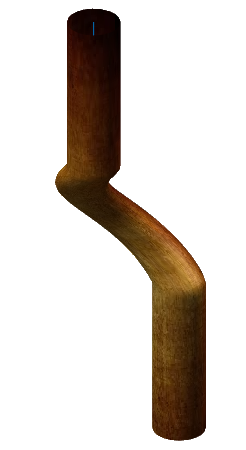
\includegraphics[width=4.5cm]{img/infor5.png}}
 	\space
 	\subfigure[Cilindro base]{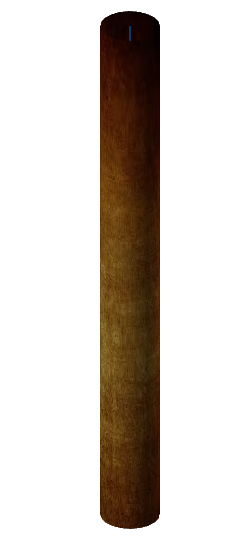
\includegraphics[width=3.8cm]{img/infor6.png}}
 	\caption{Funciones base}
 	\label{final1} 
 \end{figure}
 
 \bigskip
 Ya tenemos la estructura base que podrá tener cada sección de una cadena de una trenza. Tenemos que ser capaces de obtener las funciones que representan a las cadenas de forma completa, y no sólo por secciones. Esto lo conseguimos mediante el siguiente algoritmo:
 \begin{alg}
 	\textbf{Algoritmo param\_cadenas}(indices\_braid, n)\\
 	ENTRADA: indices\_braid (cadena de enteros que representa los cruces de una trenza)\\
 	\hspace*{2.2cm} n (número de cadenas de la trenza)\\
 	SALIDA: \hspace{0.4cm} matriz\_x (matriz que contiene las coordenadas x de las funciones que representan a las cadenas de la trenza)\\
 	\hspace*{2.2cm} matriz\_y (matriz que contiene las coordenadas y de las funciones que representan a las cadenas de la trenza)\\
 	\hspace*{2.2cm} matriz\_z (matriz que contiene las coordenadas z de las funciones que representan a las cadenas de la trenza)
 	
 	\lstset{language=Matlab, breaklines=true, basicstyle=\ttfamily\small ,numbers=left, stepnumber=1, numberstyle=\color{blue}, literate={á}{{\'a}}1
 		{í}{{\'i}}1
 		{é}{{\'e}}1
 		{ý}{{\'y}}1
 		{ú}{{\'u}}1
 		{ó}{{\'o}}1
 		{ñ}{{\~n}}1}
\begin{lstlisting}
   Aplico giro_base: obtengo vectores con coordenadas x, y, z del giro que representa una de las dos partes del cruce de una trenza. 
   Aplico cilindro_base: obtengo vectores con coordenadas x, y, z de una funcion lineal que representa una cadena sin giro. 
   Si la trenza no tiene cruces...
      anulamos las matrices x, y, z 
   Para cada cadena de la trenza (sera la cadena actual)...
      Para cada índice de índices_braid...
         Si |índice|=0 (recordemos que es posible porque lo usamos para visualizaciones mejores) -> creo vectores con coordenadas x, y, z que representan a un cilindro_base con la traslación correspondiente.
         Si |índice|=cadena actual -> creo vectores con coordenadas x, y, z que representan a un giro_base con la traslación y giro correspondiente.  
         Si |índice|=cadena actual -1 -> creo vectores con coordenadas x, y, z que representan a un giro_base con la traslación correspondiente.
         Si no -> creo vectores con coordenadas x, y, z que representan a un cilindro_base con la traslación correspondiente. 
      Genero las matrices x,y,z como concatenación de dichos vectores. 
   Si la trenza tiene cadenas a la derecha sin cruces...
      Añado para cada cadena una fila a cada matriz x, y, z con cilindros base con las traslaciones correspondientes. 
      
         
\end{lstlisting}
 \end{alg}
 
 Finalmente, vemos el algoritmo para representar una trenza cualquiera. 
\begin{alg}
  	\textbf{Algoritmo representar\_trenza}(br, N\_cortes, Radio)\\
  	ENTRADA: br (trenza)\\
  	\hspace*{2.2cm} N\_cortes (número de cortes que tendrá el tubo (cadena de la trenza))\\
  	\hspace*{2.2cm} R (Radio del tubo (cadena de la trenza))
  	
  	\lstset{language=Matlab, breaklines=true, basicstyle=\ttfamily\small ,numbers=left, stepnumber=1, numberstyle=\color{blue}, literate={á}{{\'a}}1
  		{í}{{\'i}}1
  		{é}{{\'e}}1
  		{ú}{{\'u}}1
  		{ó}{{\'o}}1
  		{ñ}{{\~n}}1}
\begin{lstlisting}
   Si número_argumentos=1 -> N_cortes=20, Radio=0.5
   Aplico param_cadenas: obtengo 3 matrices con coordenadas x, y, z de las funciones que representan las cadenas de la trenza.
   Para cada cadena de la trenza (cada fila de las matrices)...
     Represento la función de la cadena (hago un plot de la cadena a partir de la fila correspondiente de la matriz x, y, z)
     Aplico tubep a dicha cadena con N_cortes y Radio.
\end{lstlisting}
\end{alg}

 \begin{center}
 	\textbf{Algoritmo para representar una trenza cerrada.}
 \end{center} 
 En esta última sección vamos a ver el algoritmo que hemos creado para representar una trenza cerrada cualquiera. Al igual que en la sección anterior, mostramos un pseudocódigo bastante específico para que se entienda bien pues puede resultar complejo a simple vista. 
\begin{alg}
	\textbf{Algoritmo representar\_trenza}(br\_c, N\_cortes, Radio)\\
	ENTRADA: br\_c (trenza cerrada)\\
	\hspace*{2.2cm} N\_cortes (número de cortes que tendrá el tubo (cadena de la trenza))\\
	\hspace*{2.2cm} R (Radio del tubo (cadena de la trenza))
	
	\lstset{language=Matlab, breaklines=true, basicstyle=\ttfamily\small ,numbers=left, stepnumber=1, numberstyle=\color{blue}, literate={á}{{\'a}}1
		{í}{{\'i}}1
		{é}{{\'e}}1
		{ú}{{\'u}}1
		{ó}{{\'o}}1
		{ñ}{{\~n}}1}
\begin{lstlisting}
   Si número_argumentos=1 -> N_cortes=20, Radio=0.5.
   Aplico representar_trenza@trenza.
   Creo una semicircunferencia en el plano x-z.
   Aplico cilindro_base: obtengo vector con coordenadas x, y, z de una función lineal que representa una cadena sin giro.
   Para cada cadena de la trenza...
     Represento la semicircunferencia para los cierres superiores de las cadenas con los escalados y traslaciones correspondientes.
     Aplico tubep.
     Represento las cadenas para hacer los cierres a partir de cilindro_base.
     Aplico tubep.
     Represento la semicircunferencia para los cierres inferiores de las cadenas con los escalados y traslaciones correspondientes.
     Aplico tubep.
\end{lstlisting}
\end{alg}